\documentclass[12pt, oneside]{book}   	% use "amsart" instead of "article" for AMSLaTeX format
\usepackage{geometry}                		% See geometry.pdf to learn the layout options. There are lots.
\geometry{a4paper}                   		% ... or a4paper or a5paper or ... 
%\geometry{landscape}                		% Activate for rotated page geometry
%\usepackage[parfill]{parskip}    		% Activate to begin paragraphs with an empty line rather than an indent
\usepackage{graphicx}				% Use pdf, png, jpg, or eps§ with pdflatex; use eps in DVI mode
								% TeX will automatically convert eps --> pdf in pdflatex		
\usepackage{amssymb}
\usepackage{fancyhdr}
\usepackage{color}
\usepackage[latin1]{inputenc}
\usepackage{amsmath}
%SetFonts

%SetFonts
\pagestyle{fancy}
\begin{document}
\thispagestyle{empty}
\hspace{10cm}
Release date 26-02-2015
\\
\\
\begin{center}
{\huge Software Engineering 2:}
{\huge MyTaxiService}
\end{center}
\vspace*{\fill}
\begin{center}
\textbf{\huge Integration Test Plan Document} 
\\
\large{V1.0}
\end{center}
\vfill
\begin{center}
{\large Dimitar Anastasovski, Marco Colombo}
\end{center}
\clearpage
\pagestyle{plain}
\tableofcontents
\setcounter{page}{1}
\clearpage
\chapter{Introduction}
\section{Purpose}
This document will outline the system test plan that is in place and testing responsibilities. The purpose of the integration test plan is to describe the necessary tests to verify that all of the components of MyTaxiService are properly assembled.  Integration testing ensures that the unit-tested modules interact correctly
The purpose of this document is to define:
\begin{itemize}
\item The test scope, focus areas and objectives
\item The test responsibilities
\item The test strategy for the levels and types of test for this release
\item The entry and exit criteria
\item The basis of the test estimates
\item Any risks, issues, assumptions and test dependencies
\item The test schedule and major milestones
\item The test deliverables
\end{itemize}
\section{Scope}
The main accent is to simplify and optimize the access of passengers to the system and to guarantee fair management of taxi queues. We will build flexible and user-friendly web application and a mobile application that will run on Android and IOS mobile phones. This application can be used by anyone who previously will be register on the registration page. After the registration is done the user will have a user name and password that should remember for furthermore usage of the system. The passenger can call a taxi after a successful logging on the application. After that he can call a taxi and he will be informed about the code of the incoming taxi, waiting time. On the other hand taxi drivers will have a mobile application where the major purpose will be to inform the system about their availability, confirmation of a certain call and global map navigation.  City is divided into taxi zones that are uniquely associated with corresponding taxi queues for efficient usage of the system.
\section{Definitions}
\begin{tabular}{|l|l|}
\hline 
\textit{Request} & Passenger filled form for immediate ride \\
\hline 
\textit{Reservation} & Passengers can request for a vehicle at least 2 hours before the ride \\
 &and can reserve his ride \\
\hline 
\textit{User} & Is a customer who already registered and logged into the system\\
\hline 
\textit{Taxi driver} & Is a person who legally drives taxi ( with driver license and work license) \\
& already registered and logged into the system as a driver\\
\hline
\textit{System} & Is the system that has to be designed\\
\hline 
\textit{Taxi zone} & Are the zones in which the city is divided in\\
\hline
\end{tabular}
\section{Abbreviations}
No abbreviations are been used in this document
\section{Documents}
\begin{tabular}{|l|l|}
\hline
Specification document & myTaxiService Project Document\\
\hline
RASD & \textit{Requirements and Specification Document} \\
& version 1.0, November 2015 \\
\hline
DD & \textit{Design Document}, version 1.0, December 2015 \\
\hline
ITPD Example & \textit{Integration Test Plan Document Example} \\
& spinGRID, version 0.1.0, May 2006\\
\hline
\end{tabular}
\chapter{Integration strategy}
\section{Entry criteria}
\begin{tabular}{|l|l|}
\hline
\textbf{Registered Manager} \hspace{4cm} &SignUp()  \hspace{4cm} \\
& Sign In()\\
\hline
& SignIn()\\
& CancelRide()\\
\textbf{Licensed Taxi Drivers Manager}  & ViewReservation()\\
& ViewMap()\\
& SetAvailability()\\
\hline
\textbf{Unregistered User} & SignUp()\\
\hline 
& SignIn()\\
\textbf{Admin Manager} & ViewReports()\\
& BanUsers()\\
\hline
\textbf{ETA Manager} & ETA()\\
& ETAPrice()\\
\hline
\textbf{Zone Manager} & DetermineZone()\\
& AssignToAvailableDrivers()\\
\hline
\textbf{Queues Manager} & EnqueueDriver()\\
& DequeueDriver()\\
\hline
& CreateRequest()\\
\textbf{Scheduler Manager}  & FirstAvailableTaxiInQueue()\\
& DetermineZone()\\
& SendConfirmation()\\
\hline
& createReservation()\\
\textbf{Reservation Manager}  & FirstAvailableTaxiInQueue()\\
& DetermineZone()\\
& SendConfirmation()\\
\hline
\end{tabular}
\section{Integrated elements}
The following sections will describe the test cases that will be performed based on Component view diagram from DD-document . These test cases will be identified by the component that they test.
You can see the figures below:
\\
\\
\begin{figure}[h]
\centering
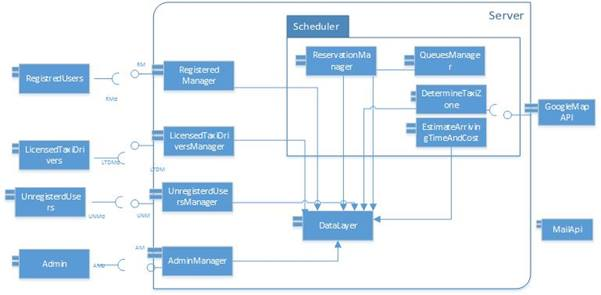
\includegraphics[scale=0.7]{Component}
\end{figure}
\\
\textbf{Figure 1: Component View}
\\
\\
\begin{figure}[h]
\centering
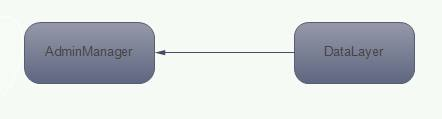
\includegraphics[scale=0.75]{AdminManager.jpg}
\end{figure}
\\
{\textbf{Figure 2: Component AdminManager}}
\\
\\
\\
\\
\\
\\
\\
\begin{figure}[h]
\centering
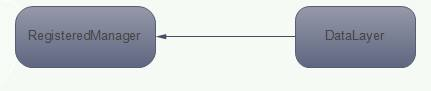
\includegraphics[scale=0.75]{RegisteredManager.jpg}
\end{figure}
\\
{\textbf{Figure 3: Component RegisteredManager}}
\\
\\
\\
\\
\begin{figure}[h]
\centering
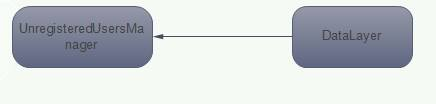
\includegraphics[scale=0.75]{UnregisteredUserManager.jpg}
\end{figure}
\\
{\textbf{Figure 4: Component UnregisteredUserManager}}
\\
\\
\\
\\
\begin{figure}[h]
\centering
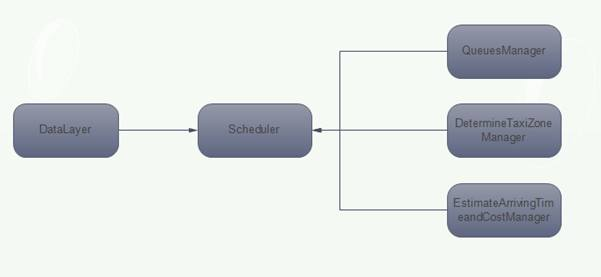
\includegraphics[scale=0.75]{Scheduler.jpg}
\end{figure}
\\
{\textbf{Figure 5: Component Scheduler}}
\clearpage
\section{Integration testing strategy}
For testing we choose a bottom-up strategy. This means that we began from the bottom levels to the top. We choose this strategy because we don't need stub and we can test all single parts before connect them together and obtain the whole project. 
The bottom-up approach implies proactive team input in the project executing process. Team members are invited to participate in every step of the management process. The decision on a course of action is taken by the whole team.
\chapter{Test specifications}
\section{Test case specifications}
\subsection{Integration test case I1T1}
\begin{tabular}{|l|l|}
\hline
Test Case Identifier & I1T1\\
\hline
Test Item & Data Layer $\rightarrow$ RegisteredManager\\
\hline
Input Specification & Create typical data layer input\\
\hline
Output Specification & Check if the correct functions are called in\\
& RegisteredManager\\
\hline
\end{tabular}
\\
\\
\subsection{Integration test case I2T1}
\begin{tabular}{|l|l|}
\hline
Test Case Identifier & I2T1\\
\hline
Test Item & Data Layer $\rightarrow$ LicensedTaxiDriverManager\\
\hline
Input Specification & Create typical data layer input\\
\hline
Output Specification & Check if the correct functions are called in\\
& LicensedTaxiDriverManager\\
\hline
\end{tabular}
\\
\\
\subsection{Integration test case I3T1}
\begin{tabular}{|l|l|}
\hline
Test Case Identifier & I3T1\\
\hline
Test Item & Data Layer $\rightarrow$ AdminManager\\
\hline
Input Specification & Create typical data layer input\\
\hline
Output Specification & Check if the correct functions are called in AdminManager\\
\hline
\end{tabular}
\\
\\
\subsection{Integration test case I4T1}
\begin{tabular}{|l|l|}
\hline
Test Case Identifier & I4T1\\
\hline
Test Item & Data Layer $\rightarrow$ UnregisteredUserManager\\
\hline
Input Specification & Create typical data layer input\\
\hline
Output Specification & Check if the correct functions are called in\\
& UnregisteredUsersManager\\
\hline
\end{tabular}
\\
\\
\subsection{Integration test case I5T1}
\begin{tabular}{|l|l|}
\hline
Test Case Identifier & I5T1\\
\hline
Test Item & QueueManager $\rightarrow$ Scheduler\\
\hline
Input Specification & Create typical Queue input\\
\hline
Output Specification & Check if the correct functions are called in Scheduler\\
\hline
\end{tabular}
\\
\\
\subsection{Integration test case I5T2}
\begin{tabular}{|l|l|}
\hline
Test Case Identifier & I5T2\\
\hline
Test Item & DetermineTaxiZoneManager $\rightarrow$ Scheduler\\
\hline
Input Specification & Create typical Zone input\\
\hline
Output Specification & Check if the correct functions are called in Scheduler\\
\hline
\end{tabular}
\\
\\
\subsection{Integration test case I5T3}
\begin{tabular}{|l|l|}
\hline
Test Case Identifier & I5T3\\
\hline
Test Item & EstimateArrivingTimeandCostManager $\rightarrow$ Scheduler\\
\hline
Input Specification & Create typical ETA input\\
\hline
Output Specification & Check if the correct functions are called in Scheduler\\
\hline
\end{tabular}
\\
\\
\subsection{Integration test case I5T4}
\begin{tabular}{|l|l|}
\hline
Test Case Identifier & I5T4\\
\hline
Test Item & Data Layer $\rightarrow$ Scheduler\\
\hline
Input Specification & Create typical Data Layer input\\
\hline
Output Specification & Check if the correct functions are called in Scheduler\\
\hline
\end{tabular}
\clearpage
\section{Test procedures}
\subsection {Test procedure T1}
\begin{tabular}{|l|l|}
\hline
Test Procedure Identifier & T1 \\
\hline
Test Items & TaxiDriver and Passenger \\
\hline
Input Specification & Create a new taxi reservation \\
\hline
Output Specification & Check if a new reservation is create \\
\hline
\end{tabular}
\\
\\
\subsection {Test procedure T2}
\begin{tabular}{|l|l|}
\hline
Test Procedure Identifier & T2 \\
\hline
Test Items & Reservation and Notify \\
\hline
Input Specification & Send notification after reservation \\
\hline
Output Specification & Check if a notification is send to the passenger \\
\hline
\end{tabular}
\\
\\
\subsection {Test procedure T3}
\begin{tabular}{|l|l|}
\hline
Test Procedure Identifier & T3 \\
\hline
Test Item & User \\
\hline
Input Specification & The user wants to log in into the system  \\
\hline
Output Specification & Check if the user is logged in succesfully\\
\hline
\end{tabular}
\\
\\
\subsection{Test procedure T4}
\begin{tabular}{|l|l|}
\hline
Test Procedure Identifier & T4 \\
\hline
Test Item & Passenger \\
\hline
Input Specification & The passemger wants to request a taxi  \\
\hline
Output Specification & Check if the passenger has called a taxi succesfully\\
\hline
\end{tabular}
\\
\\
\subsection{Test procedure T5}
\begin{tabular}{|l|l|}
\hline
Test Procedure Identifier & T5 \\
\hline
Test Item & Passenger \\
\hline
Input Specification & The passemger wants to delete a reservation \\
\hline
Output Specification & Check if the passenger has deleted the reservation\\
\hline
\end{tabular}
\\
\\
\subsection{Test procedure T6}
\begin{tabular}{|l|l|}
\hline
Test Procedure Identifier & T6 \\
\hline
Test Item & Taxi driver \\
\hline
Input Specification & The taxi driver is available \\
\hline
Output Specification & Check if the taxi driver declined or accept the request\\
\hline
\end{tabular}
\\
\\
\subsection{Test procedure T7}
\begin{tabular}{|l|l|}
\hline
Test Procedure Identifier & T7 \\
\hline
Test Items & Server and Users \\
\hline
Input Specification & The user wants to access to the application \\
\hline
Output Specification & Check if the user is already on the server\\
\hline
\end{tabular}
\\
\\
\subsection{Test procedure T8}
\begin{tabular}{|l|l|}
\hline
Test Procedure Identifier & T8\\
\hline
Test Items & Taxi and queue\\
\hline
Input Specification & The user request a taxi\\
\hline
Output Specification & Check if the taxi is available and remove from the queue\\
\hline
\end{tabular}
\\
\\
\chapter{Tools and test equipment }
To make sure that this product will be on market without unexpected behavior and can be reliable two types of testing will be done before final commercial release.
\\
\\
\textbf{Manual}
\\
\\
The main goal of manual testing is to make sure that the application under test is defect free and software application is working as per the requirement specification document (RASD). This type includes the testing of the Software manually i.e. without using any automated tool or any script. In this type, tester takes over the role of end user and test the Software to identify any un-expected behavior or bug. Manual testing will be very useful while executing test cases first time, may or may not be powerful to catch the regression defects under frequently changing requirements. This test cost less than automated one.
\\
\\
\textbf{Automatic}
\\
\\
The objective of automated testing is to simplify as much of the testing effort as possible with a minimum set of scripts. Automated testing tools are capable of executing tests, reporting outcomes and comparing results with earlier test runs. Automation testing will be used when need to execute the set of test cases tests repeatedly. This type of testing will be very useful to catch regressions in a timely manner when the code is frequently changes also will be carried out simultaneously on different machine with different OS platform combination. For this project it's going to be used:
\begin{itemize}
\item For unit testing we will use JUnit. Is a simple unit testing framework to write repeatable tests in Java. JUnit tests do not require human judgment to interpret, and it is easy to run many of them at the same time.
\item For the web application we will use Selenium. Selenium is a popular automated web testing tool and helps you automate web browsers across different platforms. Selenium has the support of some of the largest browser vendors who have taken steps to make Selenium a native part of their browser.
\item For GUI we will use Ranorex. It allows us to automate our application and  record user interactions and play them back to execute our tests. Ranorex is one of the more popular commercial tools to build and run automated GUI and web tests.
\end{itemize}
\chapter{Test data required}
We don't need any stub because we choose a bottom-up approach, but we have to use drivers to test each module and also when we connect them together.
\begin{figure}[h]
\centering
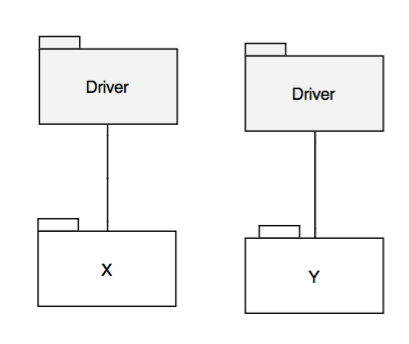
\includegraphics[scale=0.75]{modules.png}
\end{figure}
\chapter{References}
\section{Working hours}
\textbf{Dimitar Anastasovski:} $\thicksim$ hours
\\
\\
\textbf{Marco Colombo:} $\thicksim$ hours

\end{document}